\documentclass[9pt,xcolor={table}]{beamer}
\setbeamertemplate{caption}[numbered]
\usetheme[white]{Illinois}
%\title[short title]{long title}
\title[Title]{Fuel cycle needs of deploying advanced reactors}
\subtitle{UTK NE Department Colloquium}
\author[Amanda M. Bachmann]{Amanda M. Bachmann\\ Advanced Reactors and Fuel Cycles Group}
\date[04.19.2023]{April 19, 2023}
\institute[UIUC]{University of Illinois at Urbana-Champaign}


%\usepackage[table]{xcolor}
\usepackage{amsfonts}
\usepackage{amsmath}
\usepackage{xspace}
\usepackage{graphicx}
\usepackage{caption}
\usepackage{subcaption}
\usepackage{booktabs} % nice rules for tables
\usepackage{microtype} % if using PDF
\usepackage{bigints}

\graphicspath{{images/}}

\newcommand{\units}[1] {\:\text{#1}}%
\newcommand{\SN}{S$_N$}%{S$_\text{N}$}%{$S_N$}%
\newcommand{\Cyclus}{\textsc{Cyclus}\xspace} %
\newcommand{\Cycamore}{\textsc{Cycamore}\xspace} %
\DeclareMathOperator{\erf}{erf}
%I need some complimentary error functions... 
\DeclareMathOperator{\erfc}{erfc}
%Those icons in the references are terrible looking
\setbeamertemplate{bibliography item}[text]

%%%% Acronym support

\usepackage[acronym,toc]{glossaries}
\newacronym[longplural={metric tons of heavy metal}]{MTHM}{MTHM}{metric ton of heavy metal}
\newacronym{ABM}{ABM}{agent-based modeling}
\newacronym{ACDIS}{ACDIS}{Program in Arms Control \& Domestic and International Security}
\newacronym{AFCI}{AFCI}{Advanced Fuel Cycle Initiative}
\newacronym{AHTR}{AHTR}{Advanced High Temperature Reactor}
\newacronym{ANDRA}{ANDRA}{Agence Nationale pour la gestion des D\'echets RAdioactifs, the French National Agency for Radioactive Waste Management}
\newacronym{ANL}{ANL}{Argonne National Laboratory}
\newacronym{ARDP}{ARDP}{Advanced Reactors Demonstration Program}
\newacronym{API}{API}{application programming interface}
\newacronym{ARCH}{ARCH}{autoregressive conditional heteroskedastic}
\newacronym{ARE}{ARE}{Aircraft Reactor Experiment}
\newacronym{ARFC}{ARFC}{Advanced Reactors and Fuel Cycles}
\newacronym{ARMA}{ARMA}{autoregressive moving average}
\newacronym{ASME}{ASME}{American Society of Mechanical Engineers}
\newacronym{ATWS}{ATWS}{Anticipated Transient Without Scram}
\newacronym{BDBE}{BDBE}{Beyond Design Basis Event}
\newacronym{BIDS}{BIDS}{Berkeley Institute for Data Science}
\newacronym{BOL}{BOL}{Beginning-of-Life}
\newacronym{BSD}{BSD}{Berkeley Software Distribution}
\newacronym{BWR}{BWR}{Boiling Water Reactor}
\newacronym{CAFCA}{CAFCA}{ Code for Advanced Fuel Cycles Assessment }
\newacronym{CASL}{CASL}{Consortium for Advanced Simulation of Light Water Reactors}
\newacronym{CDTN}{CDTN}{Centro de Desenvolvimento da Tecnologia Nuclear}
\newacronym{CEA}{CEA}{Commissariat \`a l'\'Energie Atomique et aux \'Energies Alternatives}
\newacronym{CI}{CI}{continuous integration}
\newacronym{CNEC}{CNEC}{Consortium for Nonproliferation Enabling Capabilities}
\newacronym{CNEN}{CNEN}{Comiss\~{a}o Nacional de Energia Nuclear}
\newacronym{CNERG}{CNERG}{Computational Nuclear Engineering Research Group}
\newacronym{COSI}{COSI}{Commelini-Sicard}
\newacronym{COTS}{COTS}{commercial, off-the-shelf}
\newacronym{CSNF}{CSNF}{commercial spent nuclear fuel}
\newacronym{CTAH}{CTAHs}{Coiled Tube Air Heaters}
\newacronym{CUBIT}{CUBIT}{CUBIT Geometry and Mesh Generation Toolkit}
\newacronym{CURIE}{CURIE}{Centralized Used Fuel Resource for Information Exchange}
\newacronym{DAG}{DAG}{directed acyclic graph}
\newacronym{DANESS}{DANESS}{Dynamic Analysis of Nuclear Energy System Strategies}
\newacronym{DBE}{DBE}{Design Basis Event}
\newacronym{DESAE}{DESAE}{Dynamic Analysis of Nuclear Energy Systems Strategies}
\newacronym{DHS}{DHS}{Department of Homeland Security}
\newacronym{DOE}{DOE}{Department of Energy}
\newacronym{DOE-NE}{DOE-NE}{U.S. Department of Energy, Office of Nuclear Energy}
\newacronym{DRACS}{DRACS}{Direct Reactor Auxiliary Cooling System}
\newacronym{DRE}{DRE}{dynamic resource exchange}
\newacronym{DSNF}{DSNF}{DOE spent nuclear fuel}
\newacronym{DYMOND}{DYMOND}{Dynamic Model of Nuclear Development }
\newacronym{EBS}{EBS}{Engineered Barrier System}
\newacronym{EBR}{EBR-II}{Experimental Breeder Reactor II}
\newacronym{EDZ}{EDZ}{Excavation Disturbed Zone}
\newacronym{EG}{EG}{Evaluation Group}
\newacronym{EIA}{EIA}{U.S. Energy Information Administration}
\newacronym{EOL}{EOL}{End-of-life}
\newacronym{EPA}{EPA}{Environmental Protection Agency}
\newacronym{EP}{EP}{Engineering Physics}
\newacronym{ES}{E\&S}{Evaluation and Screening}
\newacronym{FCM}{FCM}{Fully Ceramic Microencapsulated}
\newacronym{FCO}{FCO}{Fuel Cycle Options}
\newacronym{FCT}{FCT}{Fuel Cycle Technology}
\newacronym{FCWMD}{FCWMD}{Fuel Cycle and Waste Management Division}
\newacronym{FEHM}{FEHM}{Finite Element Heat and Mass Transfer}
\newacronym{FEPs}{FEPs}{Features, Events, and Processes}
\newacronym{FHR}{FHR}{Fluoride-Salt-Cooled High-Temperature Reactor}
\newacronym{FLiBe}{FLiBe}{Fluoride-Lithium-Beryllium}
\newacronym{GCAM}{GCAM}{Global Change Assessment Model}
\newacronym{GDSE}{GDSE}{Generic Disposal System Environment}
\newacronym{GDSM}{GDSM}{Generic Disposal System Model}
\newacronym{GENIUSv1}{GENIUSv1}{Global Evaluation of Nuclear Infrastructure Utilization Scenarios, Version 1}
\newacronym{GENIUSv2}{GENIUSv2}{Global Evaluation of Nuclear Infrastructure Utilization Scenarios, Version 2}
\newacronym{GENIUS}{GENIUS}{Global Evaluation of Nuclear Infrastructure Utilization Scenarios}
\newacronym{GPAM}{GPAM}{Generic Performance Assessment Model}
\newacronym{GRSAC}{GRSAC}{Graphite Reactor Severe Accident Code}
\newacronym{GUI}{GUI}{graphical user interface}
\newacronym{HALEU}{HALEU}{High Assay Low Enriched Uranium}
\newacronym{HEU}{HEU}{High Enriched Uranium}
\newacronym{HLW}{HLW}{high level waste}
\newacronym{HPC}{HPC}{high-performance computing}
\newacronym{HTC}{HTC}{high-throughput computing}
\newacronym{HTGR}{HTGR}{High Temperature Gas-Cooled Reactor}
\newacronym{HTTR}{HTTR}{High Temperature Engineering Test Reactor}
\newacronym{IAEA}{IAEA}{International Atomic Energy Agency}
\newacronym{IEMA}{IEMA}{Illinois Emergency Mangament Agency}
\newacronym{INL}{INL}{Idaho National Laboratory}
\newacronym{IPRR1}{IRP-R1}{Instituto de Pesquisas Radioativas Reator 1}
\newacronym{IRP}{IRP}{Integrated Research Project}
\newacronym{ISFSI}{ISFSI}{Independent Spent Fuel Storage Installation}
\newacronym{ISRG}{ISRG}{Independent Student Research Group}
\newacronym{JFNK}{JFNK}{Jacobian-Free Newton Krylov}
\newacronym{LANL}{LANL}{Los Alamos National Laboratory}
\newacronym{LBNL}{LBNL}{Lawrence Berkeley National Laboratory}
\newacronym{LCOE}{LCOE}{levelized cost of electricity}
\newacronym{LDRD}{LDRD}{laboratory directed research and development}
\newacronym{LEU}{LEU}{Low Enriched Uranium}
\newacronym{LFR}{LFR}{Lead-Cooled Fast Reactor}
\newacronym{LGPL}{LGPL}{Lesser GNU Public License}
\newacronym{LLNL}{LLNL}{Lawrence Livermore National Laboratory}
\newacronym{LLW}{LLW}{low level waste}
\newacronym{LMFBR}{LMFBR}{Liquid-Metal-cooled Fast Breeder Reactor}
\newacronym{LOFC}{LOFC}{Loss of Forced Cooling}
\newacronym{LOHS}{LOHS}{Loss of Heat Sink}
\newacronym{LOLA}{LOLA}{Loss of Large Area}
\newacronym{LP}{LP}{linear program}
\newacronym{LWR}{LWR}{Light Water Reactor}
\newacronym{MARKAL}{MARKAL}{MARKet and ALlocation}
\newacronym{MA}{MA}{minor actinide}
\newacronym{MCNP}{MCNP}{Monte Carlo N-Particle code}
\newacronym{MILP}{MILP}{mixed-integer linear program}
\newacronym{MIT}{MIT}{the Massachusetts Institute of Technology}
\newacronym{MMR}{MMR}{Micro Modular Reactor}
\newacronym{MOAB}{MOAB}{Mesh-Oriented datABase}
\newacronym{MOOSE}{MOOSE}{Multiphysics Object-Oriented Simulation Environment}
\newacronym{MOX}{MOX}{mixed oxide}
\newacronym{MSBR}{MSBR}{Molten Salt Breeder Reactor}
\newacronym{MSRE}{MSRE}{Molten Salt Reactor Experiment}
\newacronym{MSR}{MSR}{Molten Salt Reactor}
\newacronym{NAGRA}{NAGRA}{National Cooperative for the Disposal of Radioactive Waste}
\newacronym{NCSA}{NCSA}{National Center for Supercomputing Applications}
\newacronym{NEAMS}{NEAMS}{Nuclear Engineering Advanced Modeling and Simulation}
\newacronym{NEUP}{NEUP}{Nuclear Energy University Programs}
\newacronym{NFCSim}{NFCSim}{Nuclear Fuel Cycle Simulator}
\newacronym{NFC}{NFC}{Nuclear Fuel Cycle}
\newacronym{NGNP}{NGNP}{Next Generation Nuclear Plant}
\newacronym{NIST}{NIST}{National Institute of Standards and Technology}
\newacronym{NMWPC}{NMWPC}{Nuclear MW Per Capita}
\newacronym{NNSA}{NNSA}{National Nuclear Security Administration}
\newacronym{NPRE}{NPRE}{Department of Nuclear, Plasma, and Radiological Engineering}
\newacronym{NQA1}{NQA-1}{Nuclear Quality Assurance - 1}
\newacronym{NRC}{NRC}{Nuclear Regulatory Commission}
\newacronym{NSF}{NSF}{National Science Foundation}
\newacronym{NSSC}{NSSC}{Nuclear Science and Security Consortium}
\newacronym{NUWASTE}{NUWASTE}{Nuclear Waste Assessment System for Technical Evaluation}
\newacronym{NWF}{NWF}{Nuclear Waste Fund}
\newacronym{NWTRB}{NWTRB}{Nuclear Waste Technical Review Board}
\newacronym{OAT}{OAT}{one-at-a-time}
\newacronym{OCRWM}{OCRWM}{Office of Civilian Radioactive Waste Management}
\newacronym{OECD}{OECD}{Organisation for Economic Cooperation and Development}
\newacronym{ORION}{ORION}{ORION}
\newacronym{ORNL}{ORNL}{Oak Ridge National Laboratory}
\newacronym{PARCS}{PARCS}{Purdue Advanced Reactor Core Simulator}
\newacronym{PBAHTR}{PB-AHTR}{Pebble Bed Advanced High Temperature Reactor}
\newacronym{PBFHR}{PB-FHR}{Pebble-Bed Fluoride-Salt-Cooled High-Temperature Reactor}
\newacronym{PEI}{PEI}{Peak Environmental Impact}
\newacronym{PH}{PRONGHORN}{PRONGHORN}
\newacronym{PI}{PI}{Principal Investigator}
\newacronym{PNNL}{PNNL}{Pacific Northwest National Laboratory}
\newacronym{PRIS}{PRIS}{Power Reactor Information System}
\newacronym{PRKE}{PRKE}{Point Reactor Kinetics Equations}
\newacronym{PSPG}{PSPG}{Pressure-Stabilizing/Petrov-Galerkin}
\newacronym{PWAR}{PWAR}{Pratt and Whitney Aircraft Reactor}
\newacronym{PWR}{PWR}{Pressurized Water Reactor}
\newacronym{PyNE}{PyNE}{Python toolkit for Nuclear Engineering}
\newacronym{PyRK}{PyRK}{Python for Reactor Kinetics}
\newacronym{QA}{QA}{quality assurance}
\newacronym{RDD}{RD\&D}{Research Development and Demonstration}
\newacronym{RD}{R\&D}{Research and Development}
\newacronym{RELAP}{RELAP}{Reactor Excursion and Leak Analysis Program}
\newacronym{RIA}{RIA}{Reactivity Insertion Accident}
\newacronym{RIF}{RIF}{Region-Institution-Facility}
\newacronym{SAM}{SAM}{Simulation and Modeling}
\newacronym{SCF}{SCF}{Software Carpentry Foundation}
\newacronym{SFR}{SFR}{Sodium-Cooled Fast Reactor}
\newacronym{SINDAG}{SINDA{\textbackslash}G}{Systems Improved Numerical Differencing Analyzer $\backslash$ Gaski}
\newacronym{SKB}{SKB}{Svensk K\"{a}rnbr\"{a}nslehantering AB}
\newacronym{SMR}{SMR}{small modular reactor}
\newacronym{SNF}{SNF}{spent nuclear fuel}
\newacronym{SNL}{SNL}{Sandia National Laboratory}
\newacronym{SNM}{SNM}{Special Nuclear Material}
\newacronym{SRS}{SRS}{Savannah River Site}
\newacronym{STC}{STC}{specific temperature change}
\newacronym{SUPG}{SUPG}{Streamline-Upwind/Petrov-Galerkin}
\newacronym{SWF}{SWF}{Separations and Waste Forms}
\newacronym{SWU}{SWU}{Separative Work Unit}
\newacronym{SandO}{S\&O}{Signatures and Observables}
\newacronym{THW}{THW}{The Hacker Within}
\newacronym{TRIGA}{TRIGA}{Training Research Isotope General Atomic}
\newacronym{TRISO}{TRISO}{Tristructural Isotropic}
\newacronym{TRU}{TRU}{transuranic}
\newacronym{TSM}{TSM}{Total System Model}
\newacronym{TSPA}{TSPA}{Total System Performance Assessment for the Yucca Mountain License Application}
\newacronym{UDB}{UDB}{Unified Database}
\newacronym{UFD}{UFD}{Used Fuel Disposition}
\newacronym{UML}{UML}{Unified Modeling Language}
\newacronym{UNFSTANDARDS}{UNFST\&DARDS}{Used Nuclear Fuel Storage, Transportation \& Disposal Analysis Resource and Data System}
\newacronym{USNC}{USNC}{Ultra Safe Nuclear Company}
\newacronym{UOX}{UOX}{uranium oxide}
\newacronym{UQ}{UQ}{uncertainty quantification}
\newacronym{US}{US}{United States}
\newacronym{UW}{UW}{University of Wisconsin}
\newacronym{VISION}{VISION}{the Verifiable Fuel Cycle Simulation Model}
\newacronym{VV}{V\&V}{verification and validation}
\newacronym{WIPP}{WIPP}{Waste Isolation Pilot Plant}
\newacronym{YMG}{YMG}{Young Members Group}
\newacronym{YMR}{YMR}{Yucca Mountain Repository Site}
\newacronym{NEI}{NEI}{Nuclear Energy Institute}
%\newacronym{<++>}{<++>}{<++>}
%\newacronym{<++>}{<++>}{<++>}

\usepackage{tikz}
\usetikzlibrary{shapes.geometric, arrows, backgrounds}
\usetikzlibrary{positioning, arrows, decorations, shapes, matrix, fit, tikzmark}

\tikzstyle{agent} = [rectangle, rounded corners, minimum width=0.1cm, minimum height=0.2cm,text centered, draw=black, fill=blue!30]
\tikzstyle{transition} = [rectangle, rounded corners, minimum width=0.1cm, minimum height=0.2cm,text centered, draw=black, fill=red!30]
\tikzstyle{arrow} = [thick,->,>=stealth]

\tikzstyle{region} = [rectangle, rounded corners, minimum width=0.1cm, minimum height=0.2cm,text centered, draw=black, fill=green!30]
\tikzstyle{institution} = [rectangle, rounded corners, minimum width=0.1cm, minimum height=0.2cm,text centered, draw=black, fill=red!30]
\tikzstyle{facility} = [rectangle, rounded corners, minimum width=0.1cm, minimum height=0.2cm,text centered, draw=black, fill=blue!30]
\tikzstyle{connect} = [thick,-]

\usepackage[beamer,customcolors]{hf-tikz}
\tikzset{hl/.style={
    set fill color=yellow!80!black!40,
    set border color=yellow!80!black,
  },
}

\def\firstcircle{(0,0) circle (2cm)}
\def\secondcircle{(60:3cm) circle (2cm)}
\def\thirdcircle{(0:3cm) circle (2cm)}
\makeglossaries

%try to get rid of header on title page\dots
\makeatletter
    \newenvironment{withoutheadline}{
        \setbeamertemplate{headline}[default]
        \def\beamer@entrycode{\vspace*{-\headheight}}
    }{}
\makeatother

\makeatother
\setbeamertemplate{footline}
{
  \leavevmode%
  \hbox{%
    \rightline{\insertframenumber{} / \inserttotalframenumber\hspace*{1ex}}
  }%
  \vskip0pt%
}
\makeatletter
\begin{document}
%%%%%%%%%%%%%%%%%%%%%%%%%%%%%%%%%%%%%%%%%%%%%%%%%%%%%%%%%%%%%
%% From uw-beamer Here's a handy bit of code to place at 
%% the beginning of your presentation (after \begin{document}):
\newcommand*{\alphabet}{ABCDEFGHIJKLMNOPQRSTUVWXYZabcdefghijklmnopqrstuvwxyz}
\newlength{\highlightheight}
\newlength{\highlightdepth}
\newlength{\highlightmargin}
\setlength{\highlightmargin}{2pt}
\settoheight{\highlightheight}{\alphabet}
\settodepth{\highlightdepth}{\alphabet}
\addtolength{\highlightheight}{\highlightmargin}
\addtolength{\highlightdepth}{\highlightmargin}
\addtolength{\highlightheight}{\highlightdepth}
\newcommand*{\Highlight}{\rlap{\textcolor{HighlightBackground}{\rule[-\highlightdepth]{\linewidth}{\highlightheight}}}}
\colorlet{lightblue}{blue!40!}
\definecolor{lightorange}{HTML}{FAA21A}
\colorlet{lightpink}{red!20!}

\tikzset{   
        every picture/.style={remember picture,baseline},
        every node/.style={anchor=base,align=center,outer sep=1.5pt},
        every path/.style={thick},
        }

\newcommand\marktopleft[1]{%
    \tikz[overlay,remember picture] 
        \node (marker-#1-a) at (.1em,.3em) {};%
}
\newcommand\markbottomright[1]{%
    \tikz[overlay,remember picture] 
        \node (marker-#1-b) at (.1em,.3em) {};%
    \tikz[overlay,remember picture,inner sep=3pt]
        \node[draw=red,rounded corners,fit=(marker-#1-a.north west) (marker-#1-b.south east)] {};%
}

%%%%%%%%%%%%%%%%%%%%%%%%%%%%%%%%%%%%%%%%%%%%%%%%%%%%%%%%%%%%%
%%--------------------------------%%
\begin{withoutheadline}
    \frame{
      \titlepage
    }
    \end{withoutheadline}

%%--------------------------------%%
\AtBeginSection[]{
\begin{frame}
  \frametitle{Outline}
  \tableofcontents[currentsection]
\end{frame}
}

\section{About Me}
\begin{frame}
    \frametitle{My background}
    Education 
    \begin{itemize}
        \item BS in Nuclear Engineering, University of Tennessee, Knoxville (2019)
        \item MS in Nuclear Engineering, University of Tennessee, Knoxville (2020)
        \item PhD in NPRE, University of Illinois Urbana-Champaign (In Progress, est. 2023)
    \end{itemize}
    Research Experience
    \begin{itemize}
        \item Multivariate modeling of radiation signatures for safeguards, using ORIGEN
        \item Modeling material flow through a pyroprocessing facility, using ORIGAMI
        \item Comparing effects of Doppler broadening methods in SHIFT (ORNL)
        \item Investigating fuel cycle impacts of using \gls{HALEU} in reactors,
              using Cyclus, Dakota, and OpenMC (UIUC/ANL)
    \end{itemize}

\end{frame}

\begin{frame}
    \frametitle{Research Interests}
    \begin{figure}[t]
    \centering
    \begin{tikzpicture}[node distance=0.6cm]
        \draw \firstcircle node[below] {};
        \draw \secondcircle node [above] {};
        \draw \thirdcircle node [below] {};
    
        % Next, we want the highlight the intersection of all three circles:
    
        %\begin{scope}
        %  \clip \firstcircle;
        %  \clip \secondcircle;
        %  \fill[green!30] \thirdcircle;
        %\end{scope}
        
        \node[align=center] at (3.5,-0.5) {Scientific\\Computing};
        \node[align=center] at (-0.5,-0.5) {Nonproliferation\\Safeguards};
        \node[align=center] at (1.5,2.75) {Nuclear\\Fuel Cycle};
        \node[align=center] at (1.5,0.84) {Me};
    \end{tikzpicture}
\end{figure}
\end{frame}
\section{Introduction}
\subsection{Motivation}
\begin{frame}
    \frametitle{The US is looking to develop supplies of HALEU}
    \begin{columns}
        \column[t]{5cm}
    \begin{itemize}
    \item Multiple new reactor designs require \gls{HALEU} fuel, which allows for: 
    \begin{itemize}
        \item Longer cycle time
        \item Increased capacity factor
        \item Higher burnup 
    \end{itemize}
    \item<2-> The US does not have any commercial supplies of \gls{HALEU}
    \item<3-> To meet the \gls{HALEU} demand, the U.S. \gls{DOE} has proposed two methods \cite{griffith_overview_2020}:
    \begin{itemize}
        \item Enrichment of natural uranium
        \item Recovery and downblending of \gls{HEU}
    \end{itemize}
    
    \end{itemize}

    \column[t]{5cm}
    \begin{table}
        \centering
        \caption{Categories of uranium enrichment by weight fraction of 
        $^{235}$U.}
        \label{tab:enrichemnt}
        \begin{tabular}{l c c}
            \hline
            Category & Weight fraction (\%)\\\hline
            Depleted & $<$0.711 \\
            Natural & 0.711 \\
            LEU & 0.711-20 \\
            \gls{HALEU} & 5-20 \\
            \gls{HEU} & $\ge$20 \\
            \hline
        \end{tabular}
    \end{table}
    \end{columns}
\end{frame}

\subsection{Background}
\begin{frame}
    \frametitle{Nuclear fuel cycle}
    \begin{figure}[t]
    \centering
    \begin{tikzpicture}[node distance=1cm]
        \node (mine) [agent] {Mine};
        \node (mill) [agent, right of=mine] {Mill};
        \node (conversion) [agent, right of=mill, xshift=0.5cm] {Conversion};
        \node (enrichment) [agent, right of=conversion, xshift=1cm]{Enrichment};
        \node (fabrication) [agent, right of=enrichment, xshift=1.5cm]{Fuel Fabrication};
        \node (reactor) [agent, below of=fabrication, yshift=-1.5cm]{Reactor};
        \node (storage) [agent,  left of=reactor, xshift=-1cm]{Storage};
        \node (sinkhlw) [agent, left of=storage, xshift=-1cm]{Repository};


        \draw [arrow] (mine) --  (mill); 
        \draw [arrow] (mill) -- (conversion); 
        \draw [arrow] (conversion) -- (enrichment);
        \draw [arrow] (enrichment) -- (fabrication);
        \draw [arrow] (fabrication) -- (reactor);
        \draw [arrow] (reactor) -- (storage);
        \draw [arrow] (storage) -- (sinkhlw);
        \pause
        \node (reprocessing) [transition, above of=storage]{Reprocessing};
        
        \draw [arrow] (storage) -- (reprocessing);
        \draw [arrow] (reprocessing) -- (fabrication);
        \draw [arrow] (reprocessing) -- (sinkhlw);
        \pause
        \node (downblending) [region, above of=fabrication]{Downblending};
        \draw [arrow] (downblending) -- (fabrication);

        \end{tikzpicture}
    \caption{Overview of the Nuclear Fuel Cycle.}
    \label{fig:fuel_cycle}
\end{figure}
\end{frame}

\begin{frame}
    \frametitle{Uranium enrichment}
    \begin{itemize}
        \item Process to increase the relative abundance of specific
              isotopes of an element
        \pause
        \item The throughput of a facility is based on the product 
              mass, product assay, and the \gls{SWU} capacity
    \end{itemize}
    \pause
    \vspace{-0.2cm}
    \begin{columns}
        \column{6.5cm}
            \begin{align*}
                    & F = P + T \\
                    & x_fF = x_pP + x_tT\\
                    & SWU = \left[P\times V(x_p) +T\times V(x_t) - F\times V(x_f)\right]*t\\
                    & \text{in which:}\\
                    & V(x_i) = (2x_i - 1)*\ln\left(\frac{x_i}{1-x_i}\right)
            \end{align*}
            \vspace{-0.5cm}
            \begin{figure}[t]
    \centering
    \begin{tikzpicture}[node distance=1cm]
        \node (conversion) [agent] {\small Conversion};
        \node (enrichment) [agent, right of=conversion, xshift=1.25cm]{\small Enrichment};
        \node (fabrication) [agent, right of=enrichment, xshift=1.25cm]{\small Fuel Fabrication};
        \node (sink) [agent, below of=enrichment]{\small Disposal};
        
        \draw [arrow] (conversion) -- node[anchor=south]{F} (enrichment);
        \draw [arrow] (enrichment) -- node[anchor=south]{P}(fabrication);
        \draw [arrow] (enrichment) -- node[anchor=east]{T}(sink);

        \end{tikzpicture}
\end{figure}
    \column{3.5cm}
    \begin{table}
        \centering
        \vspace{-0.3cm}
        \begin{tabular}{c m{2cm}}
            \hline
            Variable & Definition \\
            \hline
            F & feed mass \\
            P & product mass \\
            T & tails mass\\
            x$_i$ & assay of material stream \\
            SWU & Separative Work Units\\
            V(x$_i$) & separation potential function\\
            \hline
        \end{tabular}
    \end{table}

    \end{columns}
\end{frame}

\begin{frame}
    \frametitle{Efforts to estimate HALEU needs}
    Efforts are underway to estimate potential \gls{HALEU} needs:
    \begin{itemize}
        \item \gls{NEI} surveyed multiple reactor design companies
              to estimate \gls{HALEU} needs between now and 2035 
              \cite{korsnick_updated_2021,nuclear_energy_institute_establishing_2022}
        \item \gls{DOE} labs modeled the transition to some 
              \gls{HALEU}-fueled reactors to estimate \gls{HALEU} needs 
              to meet current net-zero carbon goals in 2050 \cite{dixon_estimated_2022}
    \end{itemize}
    \pause
    This previous work is all based on announced advanced reactor projects.
    \begin{itemize}
        \item What happens if we scale up on reactor deployment really quickly?
        \item How does decision making affect the fuel cycle requirements?
    \end{itemize}
\end{frame}

\subsection{Objectives}
\begin{frame}
    \frametitle{Objectives}
        \begin{itemize}
        \item Explore how the deployment of \gls{HALEU}-fueled reactors 
              affects the US nuclear fuel cycle
        \item Quantify potential material requirements for the transition from 
              \glspl{LWR} to advanced reactors in a once-through and recycling 
              fuel cycle
        \item Understand the impacts of fuel cycle parameters on the 
              material requirements and design optimized transition scenarios
        \item Identify potential limitations in using downblended \gls{HEU} 
              in advanced reactors
        \end{itemize}
\end{frame}
\section{Transition analysis}
\subsection{Methodology}
\begin{frame}
    \frametitle{Fuel cycle simulators}
    To quantify potential material needs, we can model the transition 
    from the current \gls{LWR} fleet to advanced reactors
    \begin{itemize}
        \item Use fuel cycle simulators to model the transition
        \item Model the deployment and decommissioning of fuel cycle facilities 
        \item Model material transactions between facilities
        \item Quantify material requirements to understand potential \gls{HALEU}
              demand
    \end{itemize}
    For this work, I am using \Cyclus \cite{huff_fundamental_2016}

\end{frame}

\begin{frame}
    \frametitle{Transition analysis assumptions}
    \begin{columns}
        
    \column[t]{6cm}
    \vspace{-0.9cm}
    \begin{figure}[t]
    \centering
    \begin{tikzpicture}[node distance=1cm]
        \node (mine) [agent] {Uranium Mine};
        \node (enrichment) [agent, below of=mine]{Enrichment};
        \node (reactor) [agent, below of=enrichment]{LWR};
        \node (adv_reactor) [transition, below of=enrichment, xshift=2cm]{Advanced Reactor};
        \node (wetstorage) [agent, below of=reactor]{Wet Storage};
        \node (sinkhlw) [agent, below of=wetstorage, xshift=0.75cm]{Repository};
        \node (sinkllw) [agent, left of=enrichment,xshift=-1cm]{Tails Sink};
        \node (adv_rx_cooling) [transition, below of=adv_reactor]{Wet Storage};

        \draw [arrow] (mine) --  (enrichment); 
        \draw [arrow] (enrichment) -- (sinkllw);
        \draw [arrow] (enrichment) -- (reactor);
        \draw [arrow] (enrichment) -- (adv_reactor);
        \draw [arrow] (reactor) -- (wetstorage);
        \draw [arrow] (wetstorage) -- (sinkhlw);
        \draw [arrow] (adv_reactor) -- (adv_rx_cooling);
        \draw [arrow] (adv_rx_cooling) -- (sinkhlw);
        \end{tikzpicture}
    \caption{Fuel cycle facilities and material flow between facilities. Facilities 
    in red are deployed at the start of the transition. }
    \label{fig:fuel_cycle}
\end{figure}

        \column[t]{4.5cm}
        Provide fuel cycle parameters to \Cyclus
        \begin{itemize}
            \item Simulations model reactor deployment from 1965-2090
            \item Transitions begin in 2025
            \item<2-> \gls{LWR} commission dates are obtained from the IAEA PRIS
                database \cite{noauthor_power_1989}
            \item<2-> \glspl{LWR} are assumed to operate until their current license 
                expires
            \item<3-> Manually calculate advanced reactor deployment
            \item<3-> Assume natural uranium is enriched to produce all 
                  fuel
        \end{itemize}

\end{columns}
\end{frame}

\begin{frame}
    \frametitle{Advanced reactors}
    \vspace{-0.2cm}
    \begingroup
        \renewcommand{\arraystretch}{1.5}
        \begin{table}
            \small
            \caption{Advanced reactor design specifications}
            \label{tab:reactor_summary}
            \vspace{-0.15cm}
            \begin{tabular}{ l p{1.5cm} p{1.5cm} p{2cm} }
                \hline
                Design Criteria & USNC MMR 
                    \cite{noauthor_usnc_2021} & 
                    X-energy Xe-100 \cite{mulder_overview_2021} & 
                    NuScale VOYGR \cite{nuscale_chapter_2020-1,reyes_nuscale_2021,reyes_correction_2022}\\\hline
                Reactor type & HTGR & HTGR & SMR\\
                Fuel type & UO$_2$ FCM & UCO TRISO & UO$_2$ pellets \\
                Power (MWe) & 5 & 80 & 77\\
                Power (MWth) & 15 & 200 & 250\\
                \tikzmarkin<2->[hl]{a}Enrichment (\% $^{235}U$) & 19.75 & 15.5 & 4.09 \\
                Cycle Length (yr) & 20 & Online & 1.5 \tikzmarkend{a}\\
                Number of cycles & 1 & 6 & 3\\
                Reactor Lifetime (yr) & 20 & 60 & 60\\
                \tikzmarkin<2->[hl]{c}Burnup ($\frac{MWd}{kg U}$) & 82 & 168 & 45\tikzmarkend{c}\\
                \hline
            \end{tabular}
        \end{table}   
    \endgroup
    \begin{equation}
        \text{mass (kg)} = \frac{\text{Power (MWth) * cycle length (d)*number of cycles}}{\text{Burnup (MWd/kg)}}
        \label{eq:fuel_mass}
    \end{equation}
\end{frame}

\begin{frame}
    \frametitle{Once-through scenario definitions}
        \begin{table}[ht]
            \centering
            \caption{Summary of the once-through fuel cycle transition scenarios.
            Energy growth is relative to energy from \glspl{LWR} in 2025.}
            \label{tab:scenarios_once-through}
            \begin{tabular}{c l l}
                \hline
                Scenario number & Reactors present & Energy demand\\\hline
                 1 & \glspl{LWR} & N/A \\
                \tikzmarkin<2->[hl]{b}2 & \glspl{LWR} and MMR & No growth \\
                3 & \glspl{LWR} and Xe-100 & No growth \\
                4 & \glspl{LWR}, Xe-100, and MMR& No growth\\
                5 & \glspl{LWR}, MMR, and VOYGR & No growth\\
                6 & \glspl{LWR}, Xe-100, and VOYGR & No growth\\
                7 & \glspl{LWR}, Xe-100, MMR, and VOYGR & No growth \tikzmarkend{b}\\
                8 & \glspl{LWR} and MMR & 1\% growth \\
                9 & \glspl{LWR} and Xe-100 & 1\% growth \\
                10 & \glspl{LWR}, Xe-100, and MMR& 1\% growth\\
                11 & \glspl{LWR}, MMR, and VOYGR & 1\% growth\\
                12 & \glspl{LWR}, Xe-100, and VOYGR & 1\% growth\\
                13 & \glspl{LWR}, Xe-100, MMR, and VOYGR & 1\% growth\\
                \hline
        \end{tabular}
        \end{table}
        %<2-> \tikz[overlay, remember picture]{\draw{draw=red,thick, double, fillopacity=0.2] ($(infrastructure)+(-0.5,0.4)$) rectangle ($(infrastructure)+(6,-0.2)$);}} 
\end{frame}

\begin{frame}
    \frametitle{Advanced reactor deployment scheme}
    \begin{columns}
        \column[t]{5cm}
            Manually calculate the deployment scheme for advanced reactors
            \begin{itemize}
                \item Preferentially deploy reactors with larger power output first
                \item Deploy reactor with largest power output until an oversupply 
                      of power would be produced, deploy the next reactor until 
                      an oversupply of power, then deploy the last reactor until 
                      demand is met
                \item Deployment schedule is given to \Cyclus
            \end{itemize}
        \column[t]{5.5cm}
            \begin{figure}
                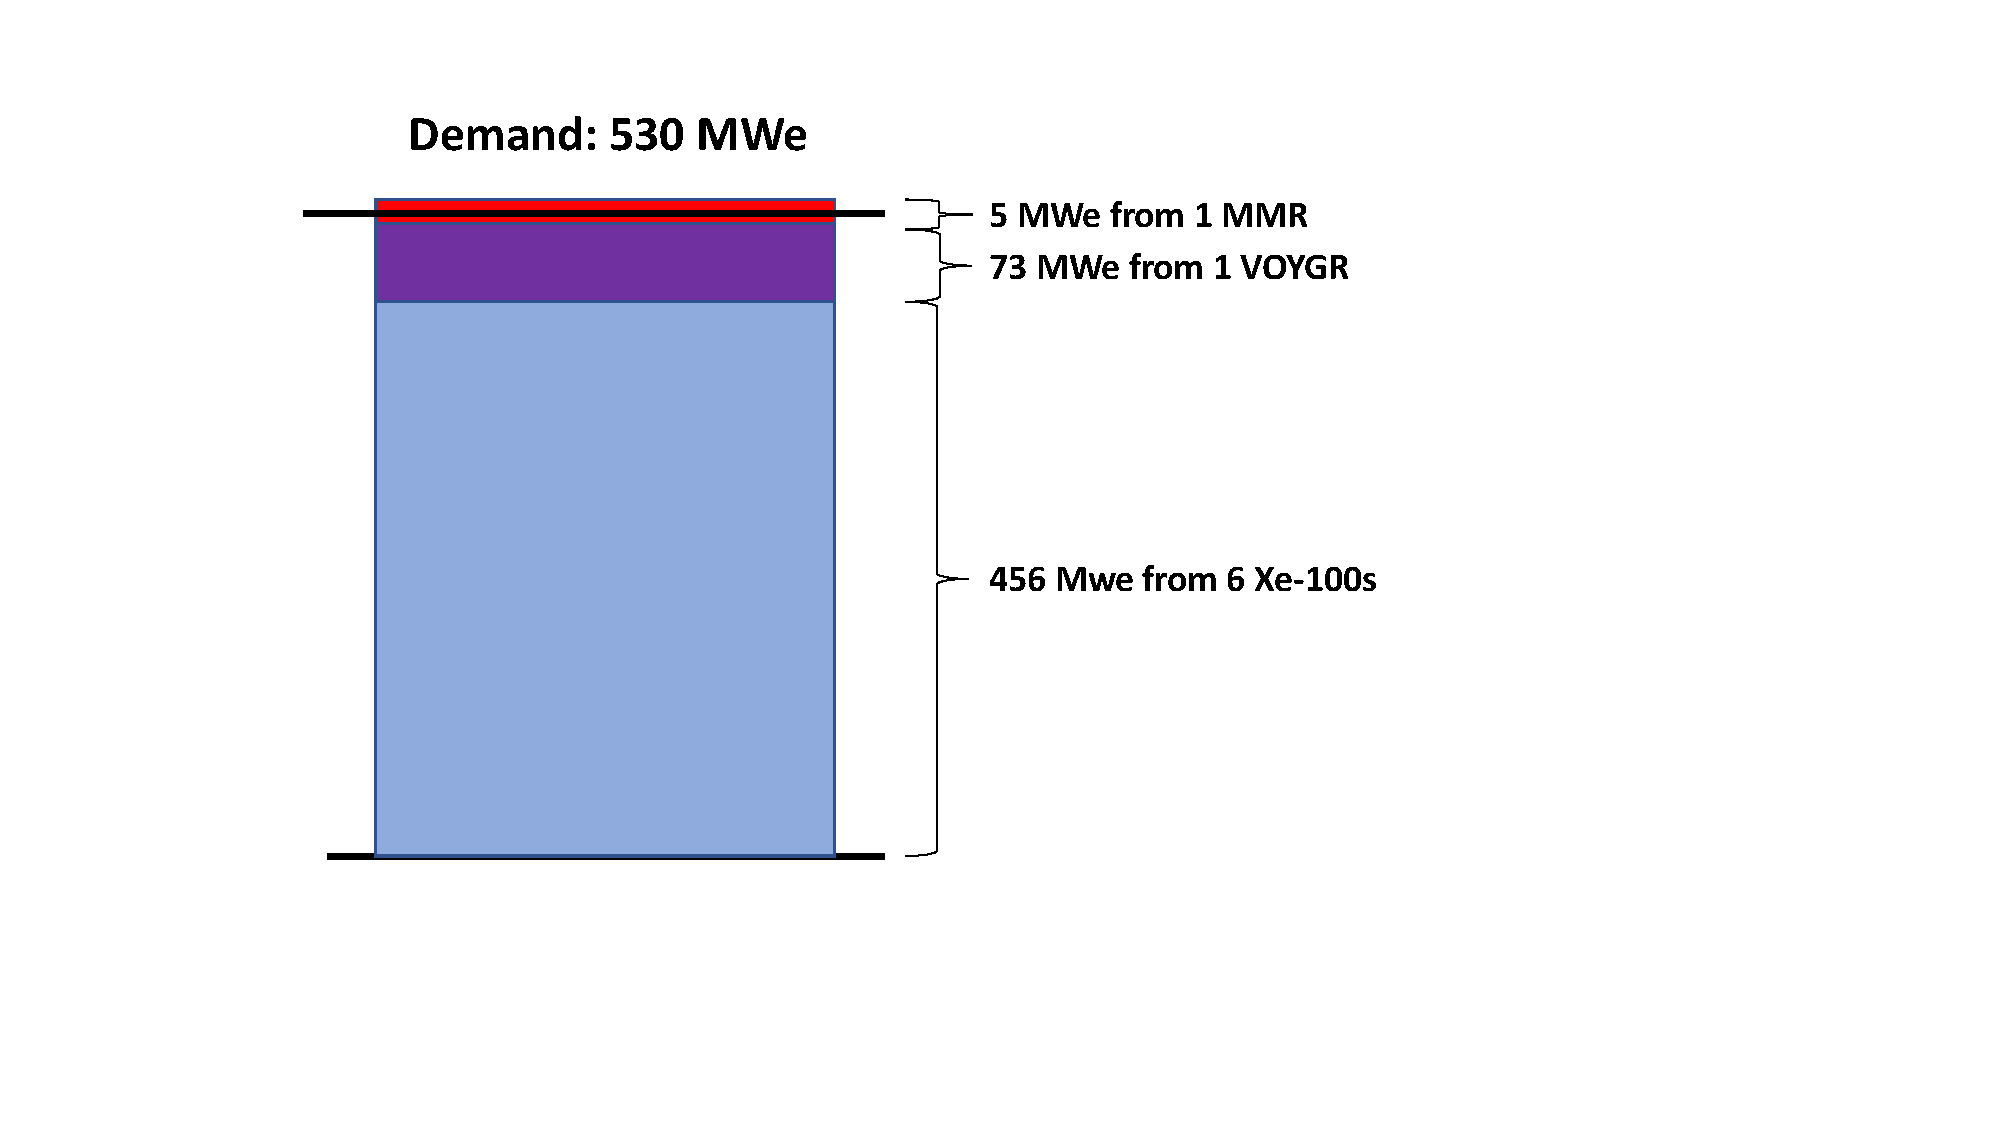
\includegraphics[scale=0.35, trim=150 100 50 50,clip]{Deployment_Scheme.pdf}
                \caption{Example of how advanced reactors in Scenario 7 are deployed to 
                meet a demand of 530 MWe.}
                \label{fig:deployment}
            \end{figure}
                    
    \end{columns}
\end{frame}
\subsection{Results}
\begin{frame}
    \frametitle{Reactor design drives the uranium mass required}
    \begin{columns}
        \column[t]{4.5cm}
            \begin{itemize}
                \item Scenario 5 (MMR + VOYGR) requires the largest average mass of 
                      enriched uranium
                \item Scenario 2 (MMR) requires the largest mass of \gls{HALEU}
                \item Scenario 3 (Xe-100) requires the smallest mass of enriched 
                      uranium
                \item Scenario 5 (MMR + VOYGR) requires the smallest mass of \gls{HALEU}
            \end{itemize}
        \column[t]{5.5cm}
        \vspace{-0.8cm}
            \begin{figure}
                \centering
                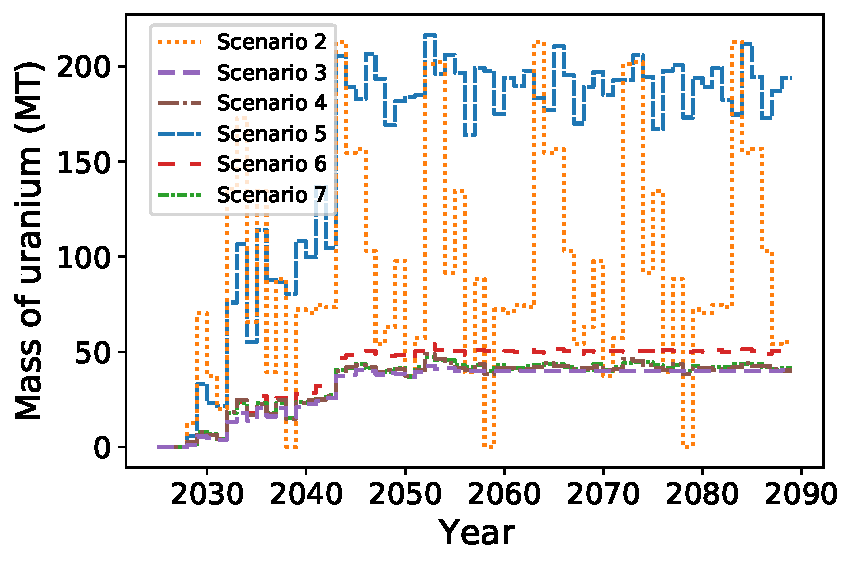
\includegraphics[scale=0.43]{nogrowth_AR_uranium.pdf}
                \caption{Annual average mass of enriched uranium required to fuel
                advanced reactors in Scenarios 2-7.}
                \label{fig:uranium}

        \end{figure}
    \end{columns}
\end{frame}

\begin{frame}
    \frametitle{\gls{SWU} capacity is a function of product mass and assay}
    \begin{columns}
        \column[t]{4.3cm}
            \begin{itemize}
                \item Scenario 2 (MMR) requires the largest average \gls{SWU} 
                \item The other scenarios are comparable for the average 
                      capacity they require
                \item This result does not capture cascade configurations or 
                      facility categories
                
            \end{itemize}
        \column[t]{5.7cm}
        \vspace{-1cm}
        \begin{figure}
                \centering
                \includegraphics[scale=0.43]{nogrowth_AR_swu.pdf}
                \caption{Annual average \gls{SWU} capacity required to produce 
                enriched uranium for and advanced reactors in Scenarios 2-7.}
                \label{fig:swu}
        \end{figure}
    \end{columns}
\end{frame}

\begin{frame}
    \frametitle{\gls{SNF} discharged follows with fuel mass}
    \begin{columns}
        \column[t]{4.3cm}
            \begin{itemize}
                \item Scenario 5 (MMR + VOYGR) discharges the largest mass of \gls{SNF}
                \item Scenario 3 (Xe-100) discharges the least \gls{SNF}
                \item Scenario 2 (MMR) discharges \gls{SNF} the latest
                \item Cumulative masses range between 25,654 MT (Scenario 3) to 
                      112,913 MT (Scenario 5)
                
            \end{itemize}
        \column[t]{5.7cm}
        \vspace{-1cm}
        \begin{figure}
                \centering
                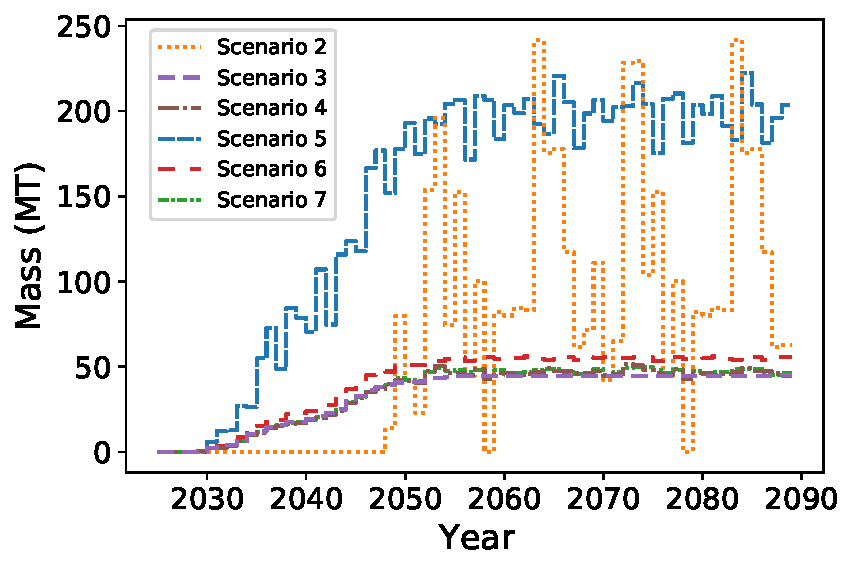
\includegraphics[scale=0.43]{nogrowth_AR_waste.pdf}
                \caption{Annual average mass of \gls{SNF} discharged from 
                advanced reactors in Scenarios 2-7.}
                \label{fig:waste}
        \end{figure}
    \end{columns}
\end{frame}

\section{Sensitivity analysis}
\subsection{Methodology}
\begin{frame}
    \frametitle{Transition analysis doesn't tell the full story}
    \begin{itemize}
        \item From the transition analysis we learned how changing which 
              reactor is predominantly built affects the material 
              requirements
        \item There are so many more parameters and assumptions in the scenario modeled
        \item We can use sensitivity analysis to see the effect of other model 
              parameters on the material requirements
    \end{itemize}
\end{frame}

\begin{frame}
    \frametitle{Sensitivity analysis provides insight into how decisions affect material needs}
    \begin{itemize}
        \item Vary a single parameter at a time and observe the output
        \item Helps to identify different relationships about the transition
        \item Couple \Cyclus with Dakota \cite{adams_dakota_2019}, model 
              variations in Scenario 7
    \end{itemize}
    \begin{columns}
        \column[t]{5cm}<2->
        Model inputs (parameters)
        \begin{itemize}
            \item Transition start time, January 2025-January 2040 
            \item LWR lifetime: percent of LWR fleet operating 
                  for 80 years, 0-50\%
            \item Build share of each advanced reactor, 0-50\%
            \item \gls{MMR} \& Xe-100 discharge burnup
        \end{itemize}

        \column[t]{5cm}<3->
        Model outputs (metrics, material requirements)
        \begin{itemize}
            \item Total fuel mass 
            \item HALEU mass
            \item Total \gls{SWU}
            \item SWU to produce HALEU
            \item Feed to produce HALEU
            \item \gls{SNF} mass
        \end{itemize}
    \end{columns}
\end{frame}

\begin{frame}
    \frametitle{Adjust deployment when varying the build share}
    \begin{columns}
        \column{4.5cm}
            \begin{itemize}
                \item Deploy the specified reactor first to meet the build share
                \item Deploy the other reactors using the previous scheme (largest 
                      to smallest power output) to meet the remaining demand
                \item Deployment schedule is given to \Cyclus
            \end{itemize}

        \column{6cm}
            \begin{figure}
                \centering 
                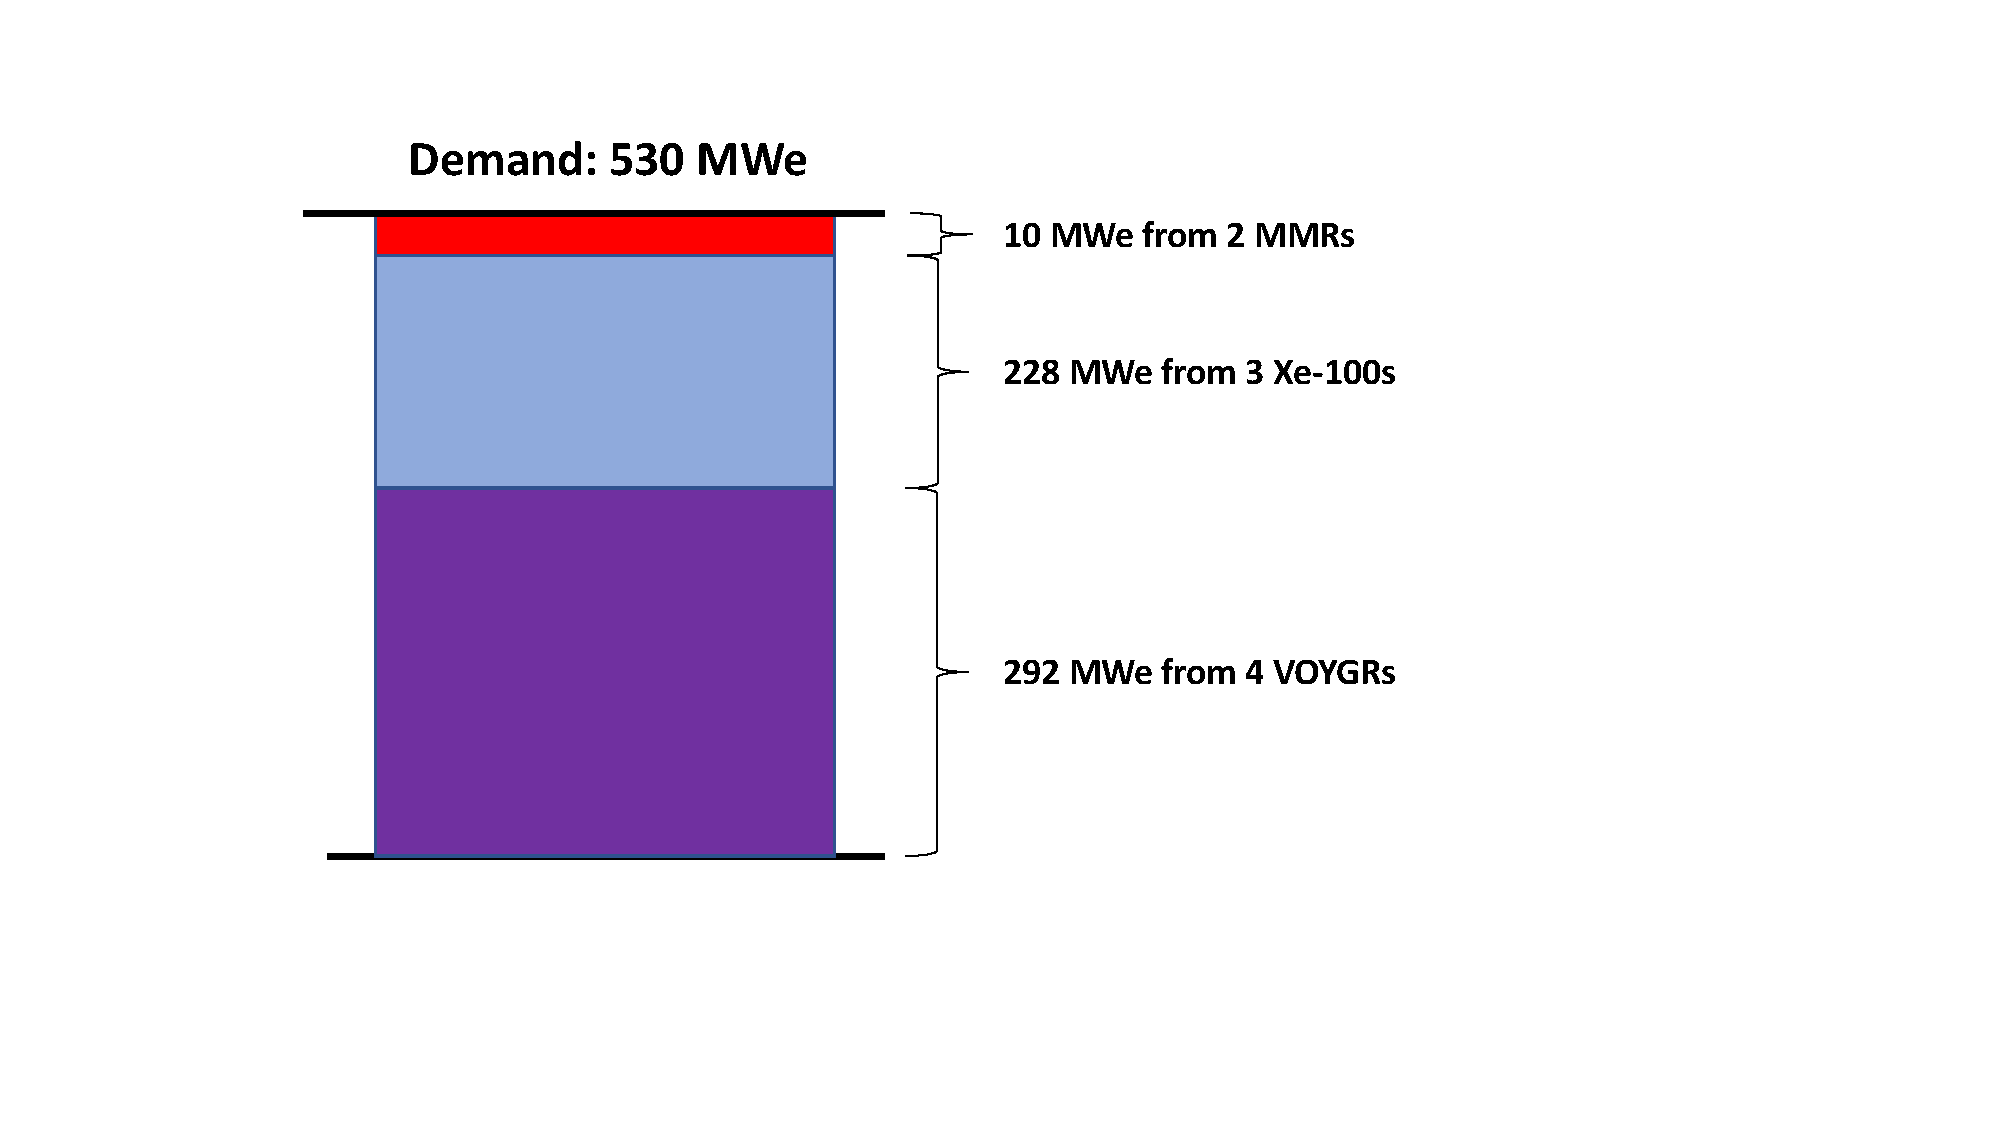
\includegraphics[scale=0.33, trim=100 100 50 50,clip]{VOYGR_build_share.pdf}
                \caption{Deployment of advanced reactors to meet 
                a demand of 530 MWe and a 50\% VOYGR build share.}
                \label{fig:build_share_deployment}
            \end{figure}
    \end{columns}
\end{frame}
\subsection{Results}
\begin{frame}
    \frametitle{Varying input: MMR build share}
    \begin{columns}
        \column{4.5cm}
            \begin{itemize}
                \item All of the metrics increase as build share increases
                \item \gls{SNF} mass has the smallest increase in 
                      relative change
                \item \gls{HALEU} \gls{SWU} capacity has the largest relative increase 
                \item These results are primarily because of the deployment scheme    
            \end{itemize}
        \column{5.5cm}
            \begin{figure}
                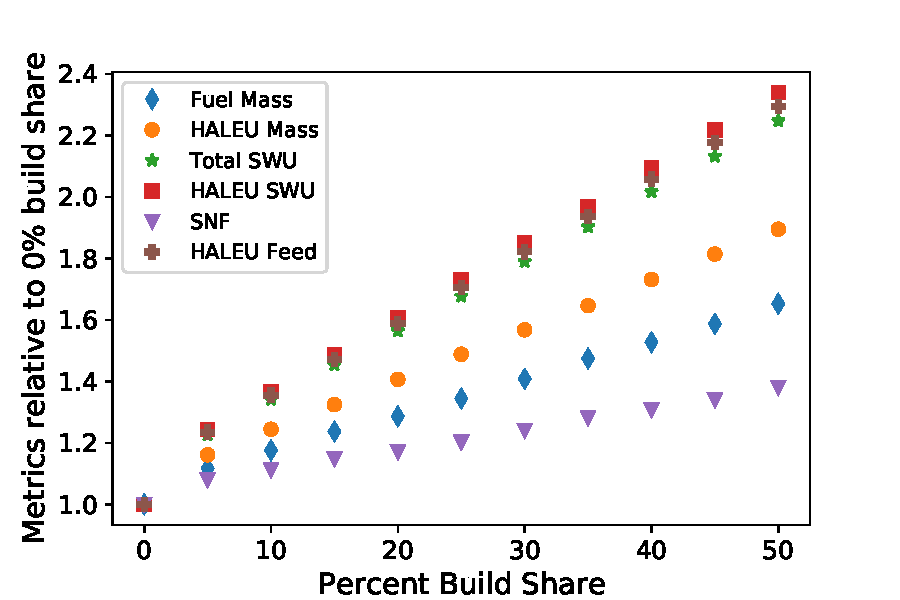
\includegraphics[scale=0.45]{mmr.pdf}
                \caption{Relative change in metrics as a function MMR 
                build share.}
                \label{fig:mmr}
            \end{figure}

\end{columns}
\end{frame}

\begin{frame}
    \frametitle{Varying MMR build share -- Number of reactors deployed}
    \begin{figure}
        \centering
        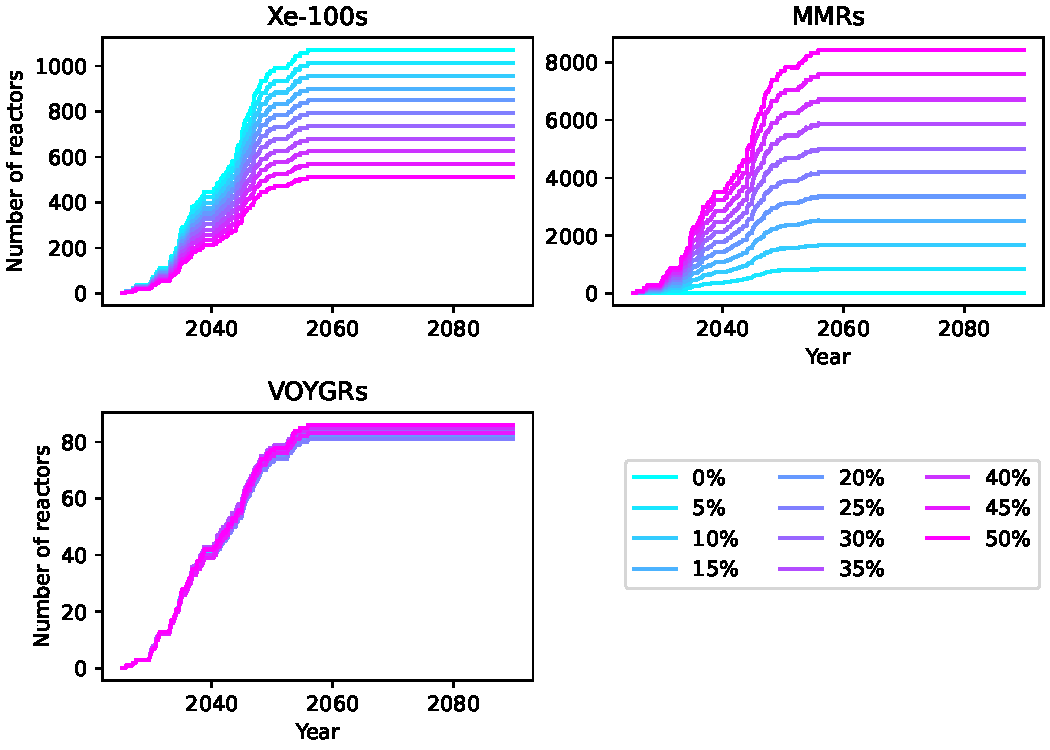
\includegraphics[scale=0.6]{mmr_combined_reactors.pdf}
        \caption{Number of MMRs deployed as a function of time when the 
        MMR build share is varied.}
    \end{figure}
\end{frame}
\begin{frame}
    \frametitle{Varying input: Xe-100 build share}
    \begin{columns}
        \column{4.5cm}
            \begin{itemize}
                \item The \gls{HALEU}-related metrics increase
                      with increasing build share
                \item Total \gls{SNF} and total fuel mass decrease with 
                      increasing build share
                \item Total \gls{SWU} capacity is relatively constant, at most 
                      a relative change of 1.06
            \end{itemize}
        \column{5.5cm}
            \begin{figure}
                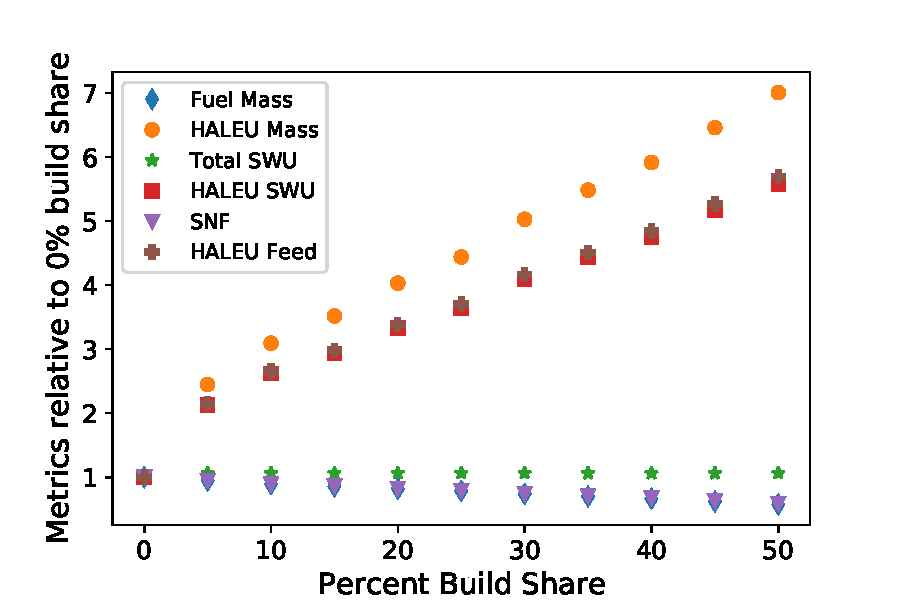
\includegraphics[scale=0.45]{xe100.pdf}
                \caption{Relative change in metrics as a function of Xe-100 
                build share \protect\cite{bachmann_sensitivity_2022}.}
                \label{fig:xe100}
            \end{figure}

\end{columns}
\end{frame}
   

\begin{frame}
    \frametitle{Varying input: VOYGR build share}
    \begin{columns}
        \column{4.5cm}
            \begin{itemize}
                \item Fuel mass and SNF mass increase while \gls{HALEU}
                      metrics decrease 
                \item Total SWU capacity is relatively constant
                \item Opposite trends as increasing Xe-100 build share
                \item As the build share increases, the number of Xe-100s
                      decreases and the number of MMRs is fairly constant
                
            \end{itemize}
        \column{5.5cm}
        \begin{figure}
            \centering 
            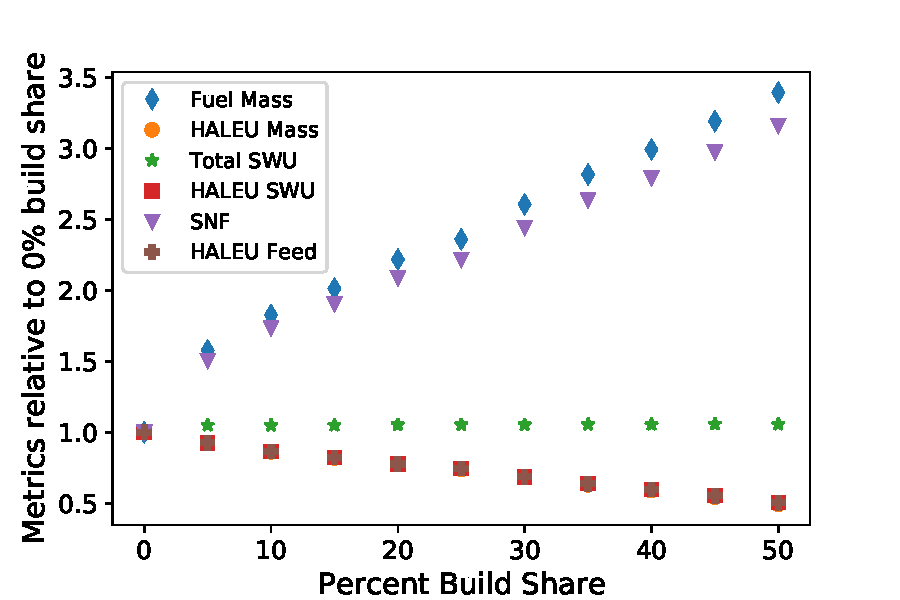
\includegraphics[scale=0.45]{voygr.pdf}
            \caption{Relative change in metrics as a function 
            of VOYGR build share \protect\cite{bachmann_sensitivity_2022}.}
            \label{fig:voygr}
        \end{figure}
    \end{columns}
\end{frame}
\section{Conclusions}
\begin{frame}
      \frametitle{Conclusions}
      \begin{itemize}
        \item Transition analysis and sensitivity analysis are methods
              to investigate the potential needs of a nuclear fuel cycle
        \item Demonstrated a methodology to investigate a fuel cycle transition
        \item<2-> The reactors deployed influence the materials needed by 
              the fuel cycle
        \item<2-> The deployment scheme strongly affects the material requirements
        \item<3-> Tradeoff between \gls{HALEU} requirements and \gls{SNF} 
              discharged between the Xe-100 and VOYGR
        \item<3-> \glspl{MMR} require more \gls{SWU} capacity, but less fuel mass
              compared with VOYGRs          
        \item<4-> All of the sensitivity analysis scenarios require a cumulative 
              \gls{HALEU} mass between 2,710 - 37,500 MT between 2025-2090       
      \end{itemize}
\end{frame}

\begin{frame}
  \frametitle{Future Work}
  \begin{block}{Ongoing Work}
    
  \begin{itemize}
    \item Consider recycling scenarios (close the fuel cycle)
    \begin{itemize}
      \item Couple \Cyclus with OpenMC's depletion solver
    \end{itemize}
    \item Perform optimization of these fuel cycles to minimize material
          requirements.
    \item Investigate some of the effects of using downblended uranium 
          in advanced reactors
  \end{itemize}
  \end{block}

  \pause
  \begin{block}{Future Work}
    \begin{itemize}
      \item Convert these mass/capacity needs to facility sizes and numbers
      \item Investigate costs for developing facilities
      \item Apply limits on uranium sources and facility throughputs
      \item<1-> Investigate safeguards for advanced reactor fuel cycles
      \item<1-> Research fast reactors, their fuel cycle, and safeguards for them
    \end{itemize}
  \end{block}
\end{frame}
\begin{frame}
    \frametitle{Acknowledgements}
    This material is based upon work supported under a University 
        Nuclear Leadership Program Graduate Fellowship. Any opinions, findings, conclusions, or 
    recommendations expressed in this publication are those of the author(s) 
    and do not necessarily reflect the views of the Department of Energy Office 
    of Nuclear Energy.
        
    I would also like to thank:
    \begin{itemize}
        \item Madicken Munk
        \item Scott Richards
        \item Bo Feng
        \item TK Kim
        \item RFCA/ARFC Group members
    \end{itemize}

\end{frame}


\begin{frame}[allowframebreaks]
    \frametitle{References}
    \bibliographystyle{plain}
    {\footnotesize \bibliography{bibliography} }
  
\end{frame}

\begin{frame}
  \large Questions?
\end{frame}

\begin{frame}
    \frametitle{Enriched uranium masses}
    \begin{table}
        \centering 
        \caption{Metrics for enriched uranium sent to advanced 
        reactors between 2025-2090 in Scenarios 2-7.}
        \label{tab:nogrowth_uranium}
        \begin{tabular}{l p{2cm} p{2cm} p{2cm} p{2cm}}
            \hline
            Scenario & Average (MT/month) & \gls{HALEU} Average 
            (MT/month) & Maximum (MT)& Cumulative (MT)\\\hline
            2 & 88.90 & 88.90 & 1,007 & 69,251\\
            3 & 31.64 & 31.64 & 86.79 & 24,646\\
            4 & 33.62 & 33.62 & 101.5 & 26,193\\
            5 & 152.3 & 3.070 & 581.1 & 118,608\\
            6 & 39.92 & 29.51 & 103.3 & 31,095\\
            7 & 33.85 & 32.97 & 103.0 & 26,370\\
            \hline
        \end{tabular}
    \end{table}
\end{frame}

\begin{frame}
    \frametitle{SWU capacity}
    \begin{table}
        \centering 
        \caption{Metrics for \gls{SWU} capacity to enrich uranium for 
        advanced reactors between 2025-2090 in Scenarios 2-7.}
        \label{tab:nogrowth_swu}
        \begin{tabular}{l p{2cm} p{2cm} p{2cm}}
            \hline
            Scenario & Average  (MT-SWU/month) & Average
            for \gls{HALEU} (MT-SWU/month) & Maximum (MT-SWU)\\\hline
            2 & 4,010 & 4,010 & 45,424 \\
            3 & 1,090 & 1,090 & 2,991\\
            4 & 1,192 & 1,192 & 3,668\\
            5 & 1,145 & 138.5 & 4,228 \\
            6 & 1,087 & 1,017 & 3,050\\
            7 & 1,167 & 1,161 & 3,735\\
            \hline
        \end{tabular}
    \end{table}
\end{frame}

\begin{frame}
    \frametitle{SNF discharged}
    \begin{table}
        \centering 
        \caption{Metrics for waste discharged from advanced reactors 
        between 2025-2090 in Scenarios 2-7.}
        \label{tab:nogrowth_waste}
        \begin{tabular}{l p{2cm} p{2cm} p{2cm} p{2cm}}
            \hline
            Scenario & Average (MT/month) & Average of \gls{HALEU} 
            (MT/month) & Maximum (MT) & Cumulative (MT)\\\hline
            2 & 66.15 & 66.15 & 1,142 & 51,531\\
            3 & 32.93 & 32.93 & 55.29 & 25,654\\
            4 & 34.07 & 34.07 & 77.55 & 26,543\\
            5 & 144.9 & 2.294 & 377.0 & 112,913\\
            6 & 40.68 & 30.72 & 75.12 & 31,691\\
            7 & 34.46 & 33.62 & 83.14 & 26,848\\
            \hline
        \end{tabular}
    \end{table}

\end{frame}

\begin{frame}
    \frametitle{Transition Start Time}
    \begin{figure}
        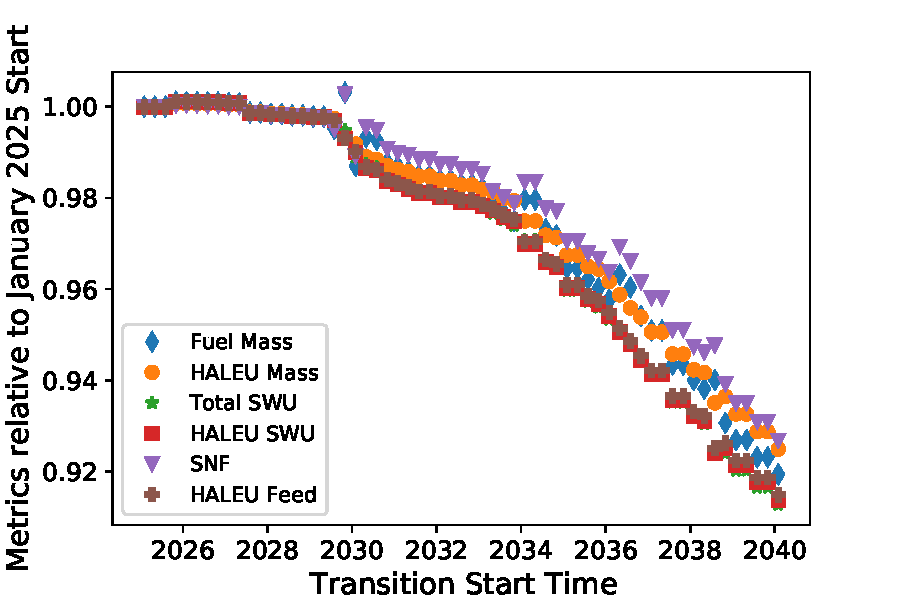
\includegraphics[scale=0.5]{ts.pdf}
        \caption{Change in metrics from varying the transition start time.}
        \label{fig:ts}
    \end{figure}
\end{frame}

\begin{frame}
    \frametitle{LWR Lifetime}
    \begin{figure}
        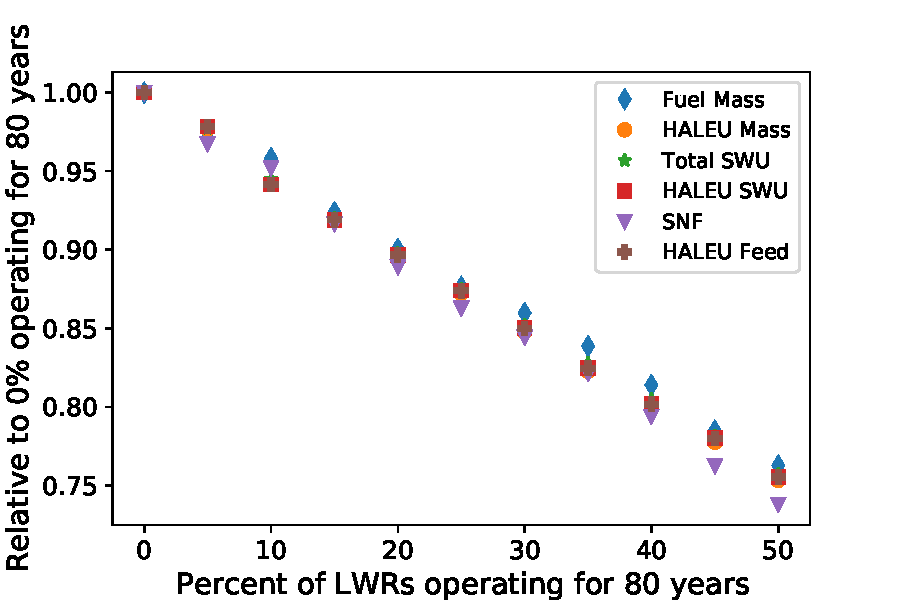
\includegraphics[scale=0.5]{lwr.pdf}
        \caption{Change in metrics from varying the percent of 
        the LWR fleet operating for 80 years.}
        \label{fig:lwr}
    \end{figure}
\end{frame}

\begin{frame}
    \frametitle{MMR Burnup}
    \begin{figure}
        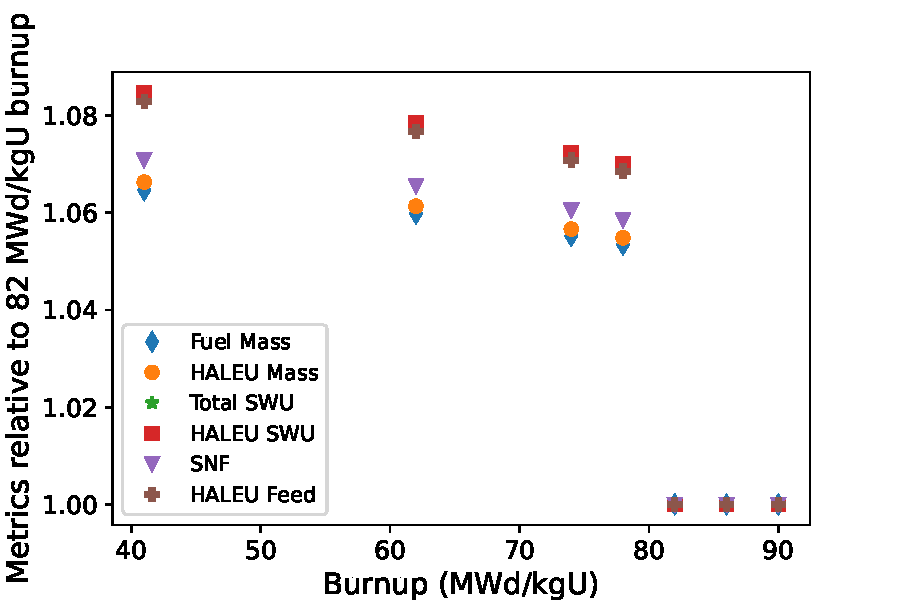
\includegraphics[scale=0.5]{mmr_bu.pdf}
        \caption{Change in metrics from varying the MMR burnup.}
        \label{fig:mmr_bu}
    \end{figure}
\end{frame}


\begin{frame}
    \frametitle{Xe-100 burnup}
    \begin{figure}
        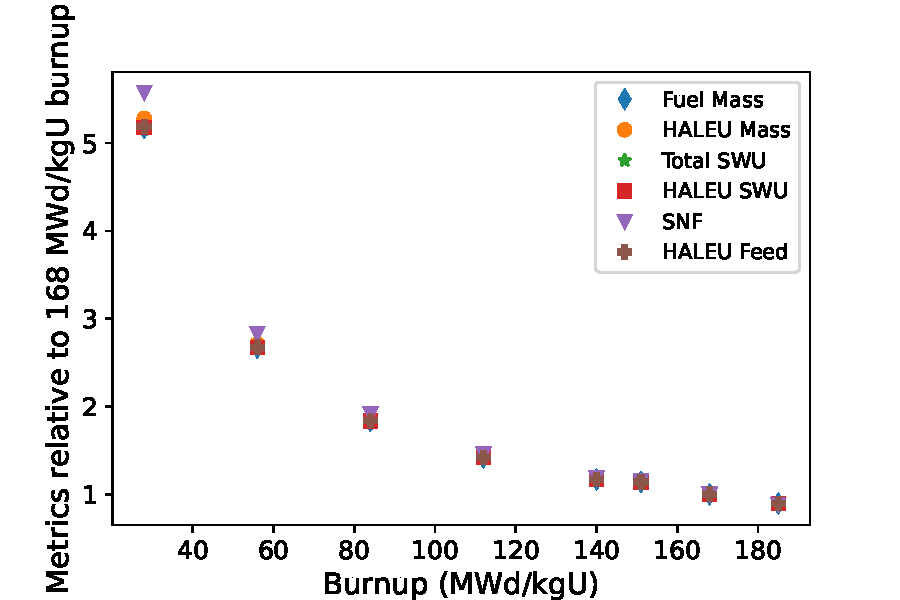
\includegraphics[scale=0.5]{xe100_bu.pdf}
        \caption{Change in metrics from varying the Xe-100 burnup.}
        \label{fig:xe100_bu}
    \end{figure}
\end{frame}


\end{document}
